
\section{Exterritoriale Stationen}
\label{section:exterritoriale_stationen}
\begin{frame}%STARTCONTENT

\begin{columns}
    \begin{column}{0.48\textwidth}
    \begin{itemize}
  \item Amateurfunkstelle außerhalb des Hoheitsgebiets der BRD
  \item Und kein anderes Land hat an diesem Standort ein Hoheitsgebiet
  \item Rufzeichen aus dem Block DP0AA bis DP2ZZ
  \end{itemize}

    \end{column}
   \begin{column}{0.48\textwidth}
       
\begin{figure}
    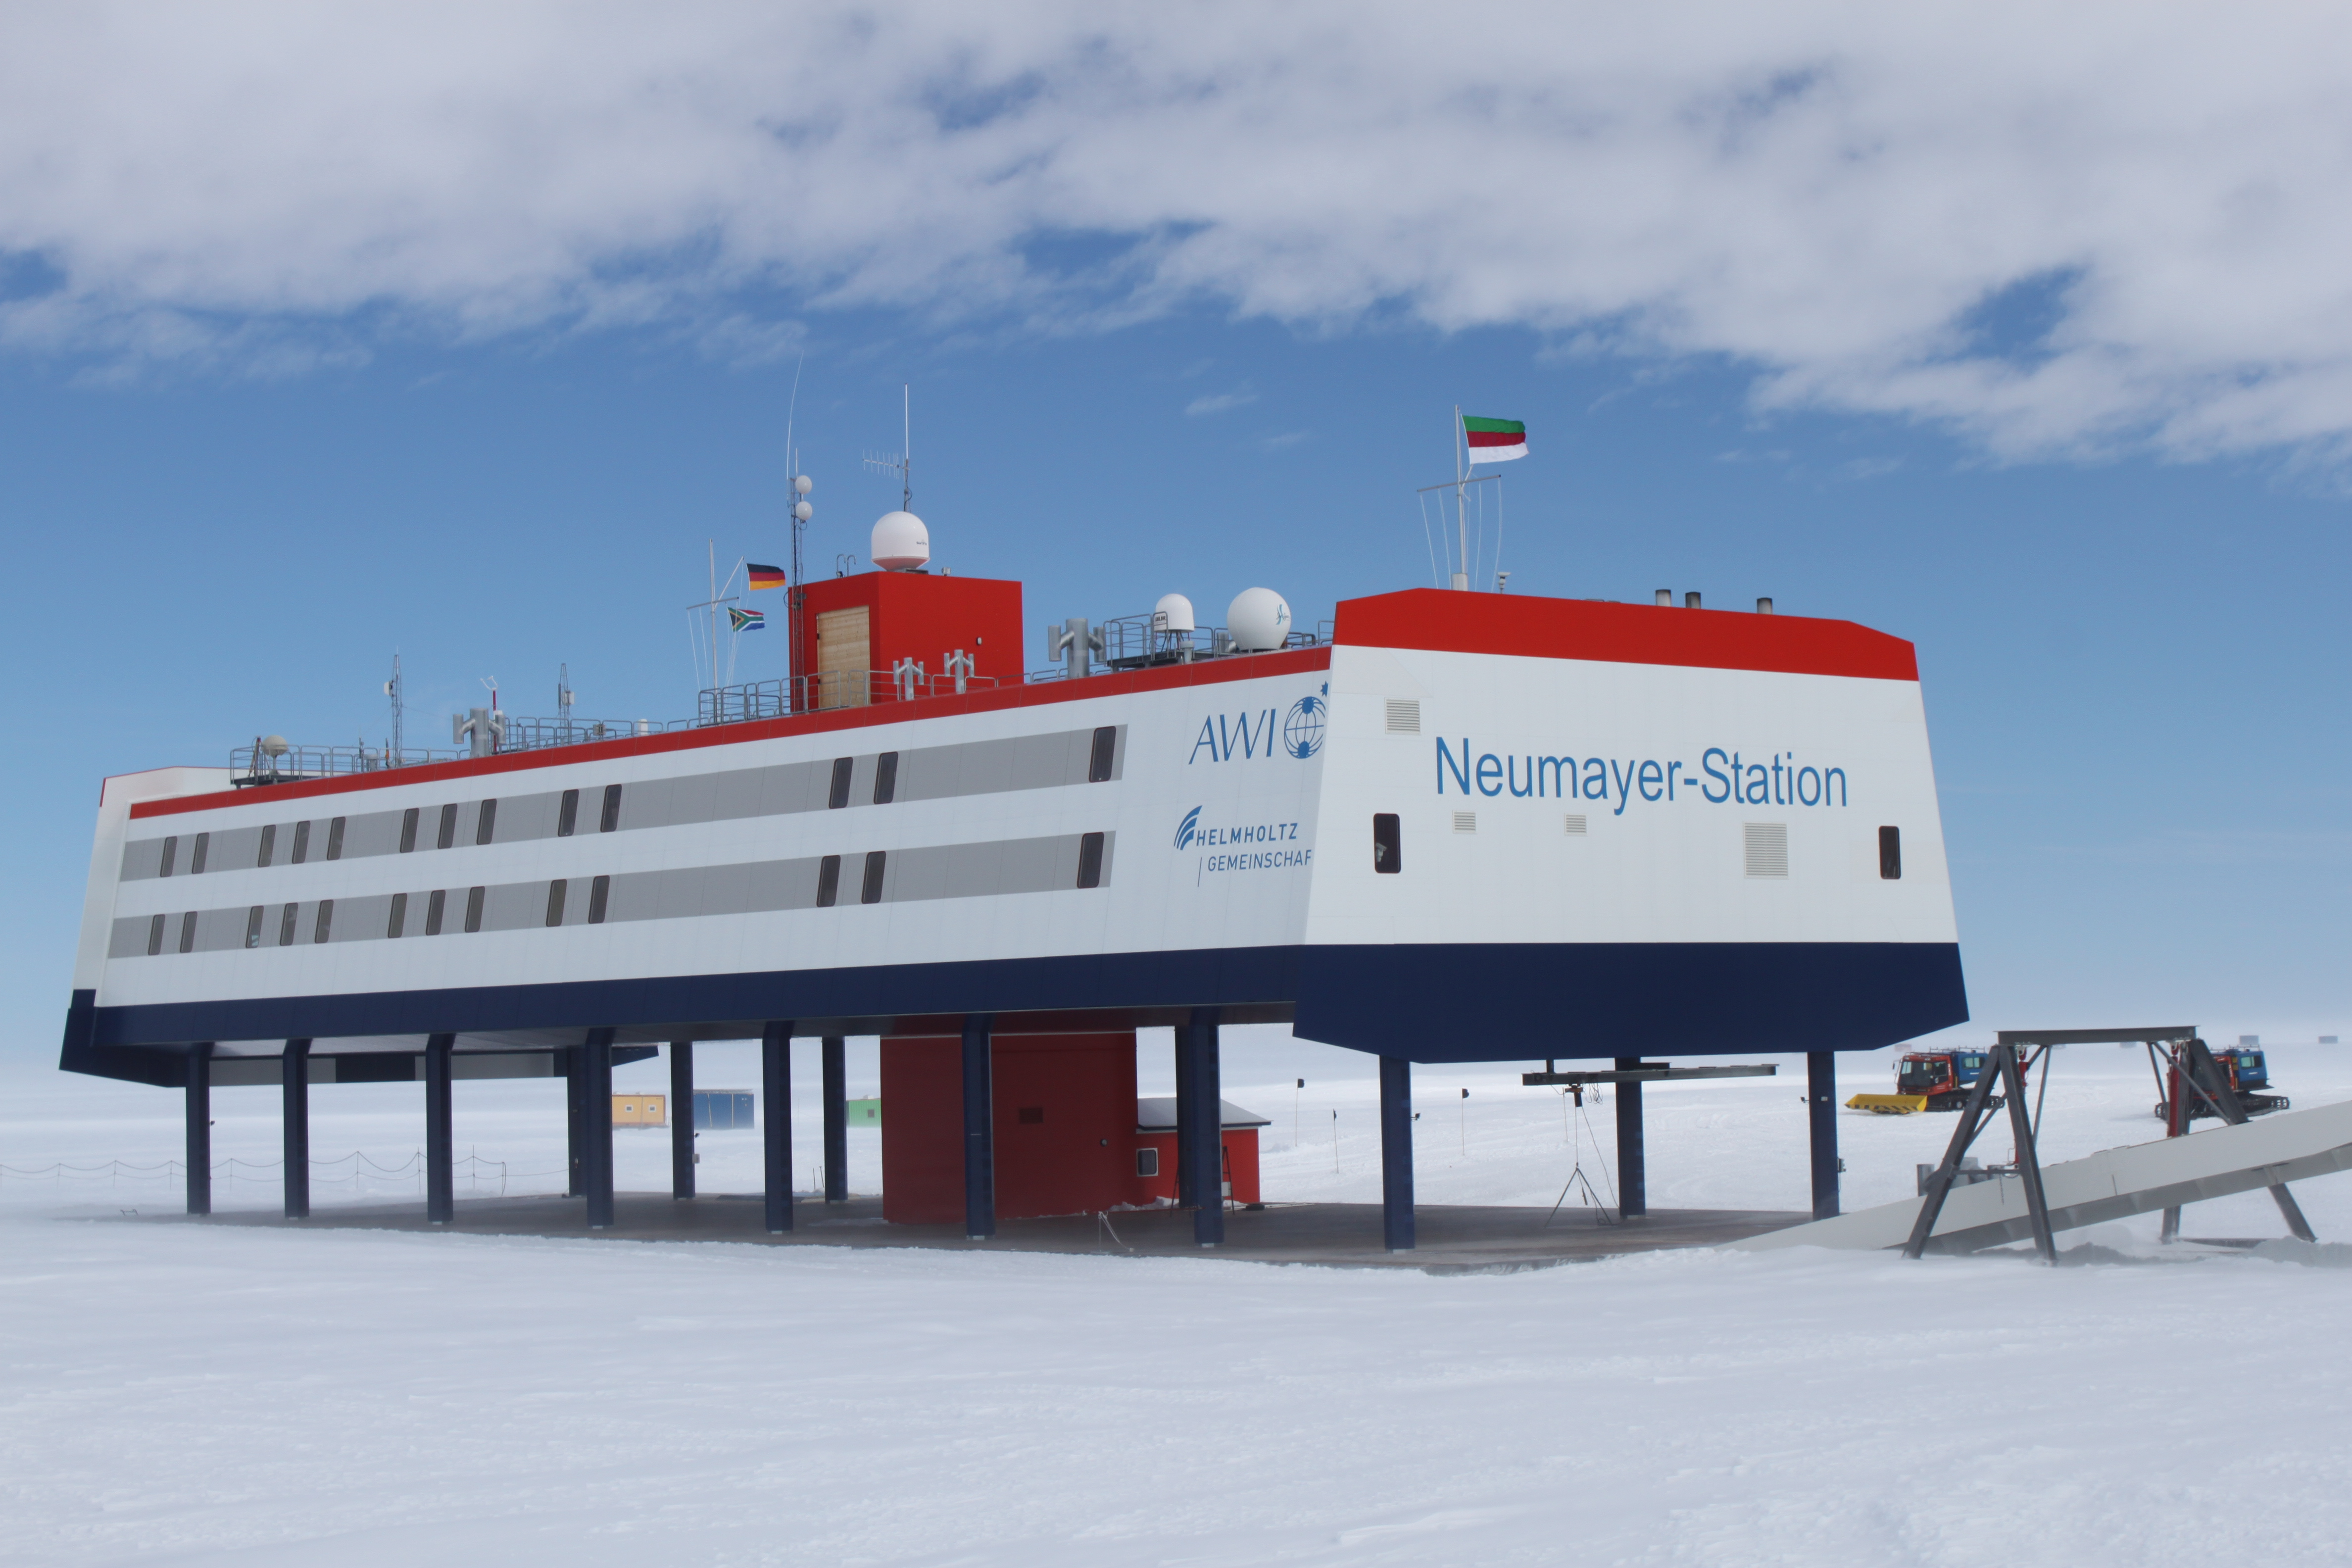
\includegraphics[width=0.85\textwidth]{foto/126}
    \caption{\scriptsize Auf der Polarforschungsstation Neumayer III befindet sich die Amateurfunkstation DP0GVN.}
    \label{n_exterritoriale_stationen_neumeyer_station}
\end{figure}

   \end{column}
\end{columns}

\end{frame}

\begin{frame}
\begin{columns}
    \begin{column}{0.48\textwidth}
    Beispiele:

\begin{itemize}
  \item Internationale Raumstation (ISS): DP0ISS
  \item Neumayer~III-Forschungsstation in der Antarktis: DP0GVN
  \item Forschungsschiff Polarstern: DP0POL
  \end{itemize}

    \end{column}
   \begin{column}{0.48\textwidth}
       
\begin{figure}
    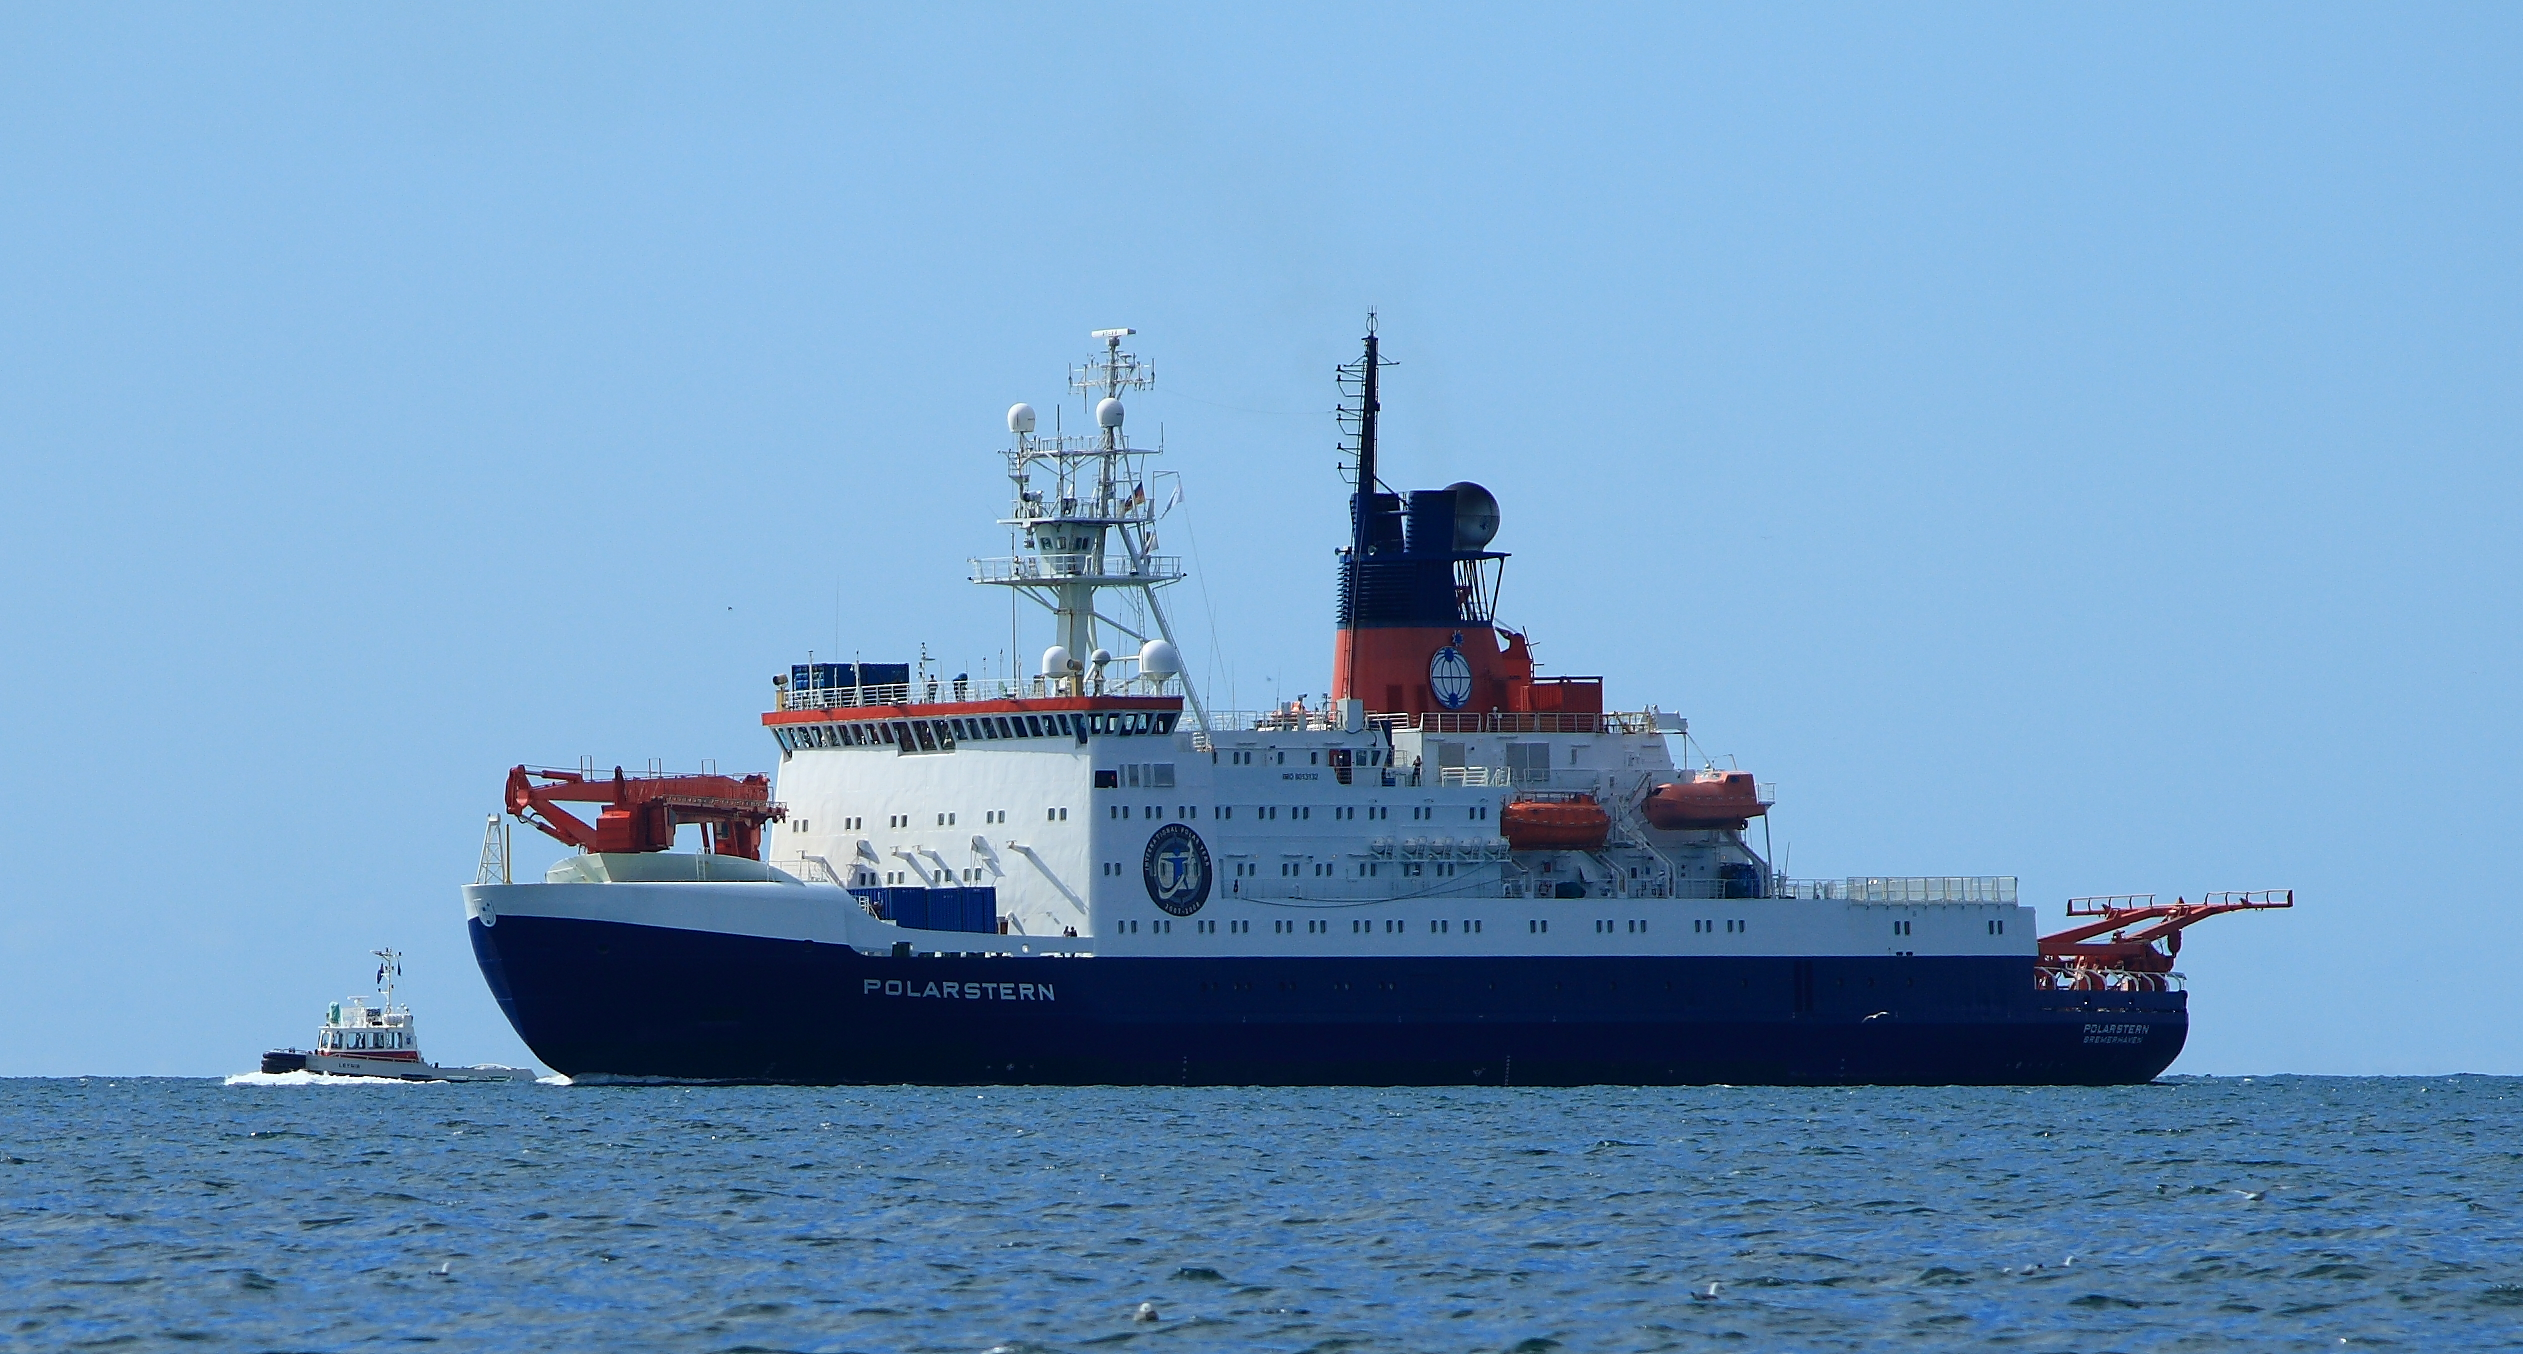
\includegraphics[width=0.85\textwidth]{foto/125}
    \caption{\scriptsize Die Amateurfunkstation an Bord des Forschungsschiff Polarstern verwendet das Rufzeichen DP0POL.}
    \label{n_exterritoriale_stationen_polarstern}
\end{figure}

   \end{column}
\end{columns}

\end{frame}

\begin{frame}
\only<1>{
\begin{QQuestion}{BD107}{Sie hören die Station DP0GVN. Um welche Art von Amateurfunkstelle handelt es sich? Es handelt sich um eine~...}{Amateurfunkstelle der Klasse A, die exterritorial betrieben wird.}
{Amateurfunkstelle der Klasse E, die ohne Anzeige nach BEMFV betrieben werden darf.}
{Klubstation der Klasse A von Funkamateuren, die Angehörige der Gaststreitkräfte in Deutschland sind.}
{Amateurfunkstelle der Klasse E, die exterritorial betrieben wird.}
\end{QQuestion}

}
\only<2>{
\begin{QQuestion}{BD107}{Sie hören die Station DP0GVN. Um welche Art von Amateurfunkstelle handelt es sich? Es handelt sich um eine~...}{\textbf{\textcolor{DARCgreen}{Amateurfunkstelle der Klasse A, die exterritorial betrieben wird.}}}
{Amateurfunkstelle der Klasse E, die ohne Anzeige nach BEMFV betrieben werden darf.}
{Klubstation der Klasse A von Funkamateuren, die Angehörige der Gaststreitkräfte in Deutschland sind.}
{Amateurfunkstelle der Klasse E, die exterritorial betrieben wird.}
\end{QQuestion}

}
\end{frame}

\begin{frame}
\only<1>{
\begin{QQuestion}{BD108}{Sie hören die Station DP0POL. Um welche Art von Amateurfunkstelle handelt es sich? Es handelt sich um eine Amateurfunkstelle~...}{von Angehörigen der Gaststreitkräfte in Deutschland.}
{der Klasse E, die ohne Anzeige nach BEMFV betrieben werden darf.}
{eines ausländischen Funkamateurs, der eine Amateurfunkprüfungsbescheinigung, aber kein individuelles Rufzeichen hat.}
{der Klasse A, die an einem exterritorialen Standort betrieben wird.}
\end{QQuestion}

}
\only<2>{
\begin{QQuestion}{BD108}{Sie hören die Station DP0POL. Um welche Art von Amateurfunkstelle handelt es sich? Es handelt sich um eine Amateurfunkstelle~...}{von Angehörigen der Gaststreitkräfte in Deutschland.}
{der Klasse E, die ohne Anzeige nach BEMFV betrieben werden darf.}
{eines ausländischen Funkamateurs, der eine Amateurfunkprüfungsbescheinigung, aber kein individuelles Rufzeichen hat.}
{\textbf{\textcolor{DARCgreen}{der Klasse A, die an einem exterritorialen Standort betrieben wird.}}}
\end{QQuestion}

}
\end{frame}%ENDCONTENT
